\documentclass[tikz,border=6pt]{standalone}
\usepackage{pgfplots}
\pgfplotsset{compat=1.18}
\usepgfplotslibrary{colormaps}
\usetikzlibrary{arrows, arrows.meta, calc}
\usetikzlibrary{decorations.markings}


\usepackage{amssymb,amsmath,mathtools}

\usepackage[T1]{fontenc}
\usepackage[utf8]{inputenc}
\usepackage{newpxtext,newpxmath}
\usepackage{sectsty}

\renewcommand{\Re}{\operatorname{\mathrm{Re}}}
\renewcommand{\Im}{\operatorname{\mathrm{Im}}}

\begin{document}
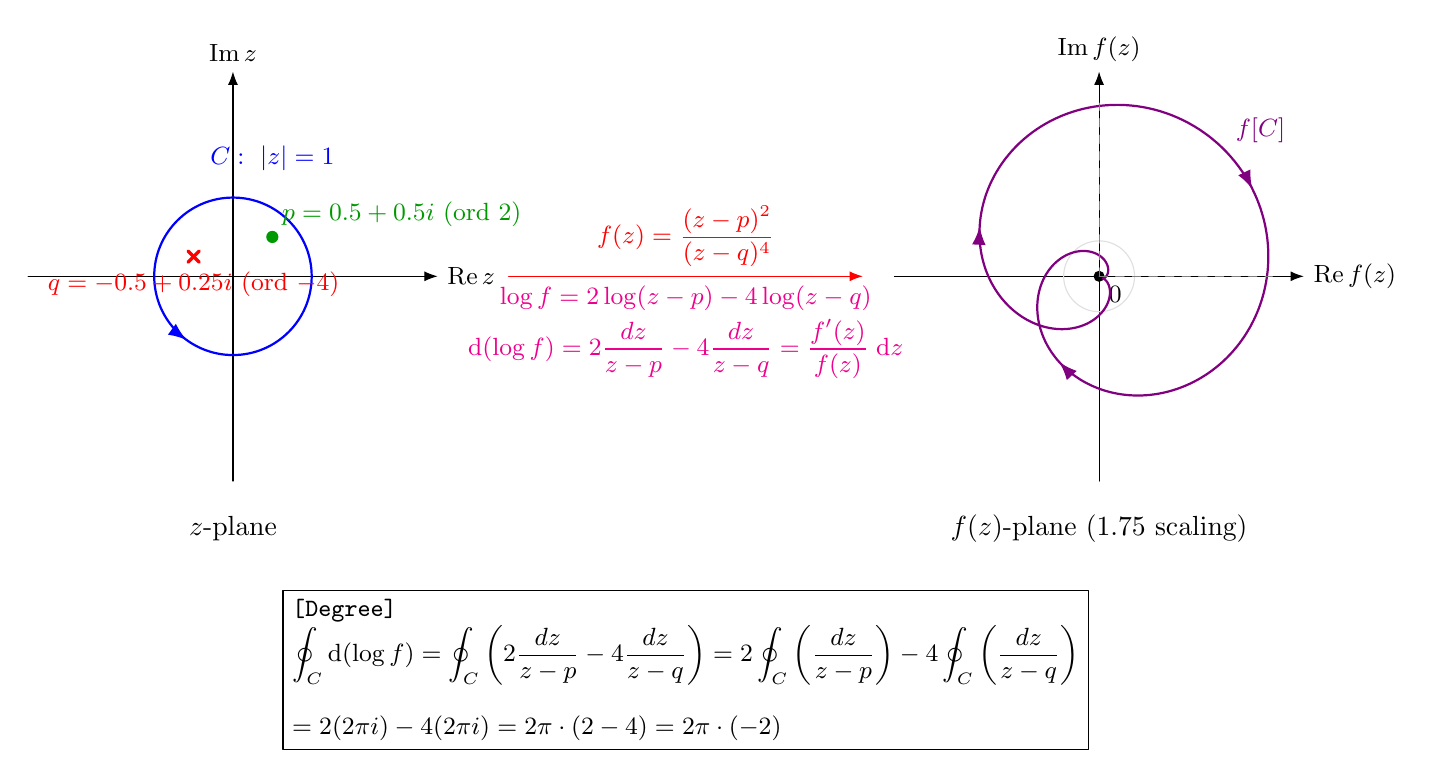
\begin{tikzpicture}[>=Latex, line cap=round, line join=round, font=\small]
%========================
% Left: z-plane
%========================
\begin{scope}[shift={(0,0)}]
	\node[font=\normalsize] at (0,-3.2) {$z$-plane};
	% axes
	\draw[->] (-2.6,0)--(2.6,0) node[right] {$\Re z$};
	\draw[->] (0,-2.6)--(0,2.6) node[above] {$\Im z$};
	% unit circle C (positively oriented) -- radius 1.5
	\draw[blue,thick,postaction={decorate},
	decoration={markings, mark=at position 0.65 with {\arrow{>}}}]
	(0,0) circle (1);
	\node[blue] at (0.5,1.5) {$C:\ |z|=1$};
	
	% pick small non-real p, q so f(C) stays near your prior picture
	% p = 0.5 + 0.5 i,  q = -0.5 + 0.25 i
	\fill[green!60!black] (0.5,0.5) circle(2.2pt) node[above right] {$p=0.5+0.5i$ (ord $2$)};
%	\node[green!60!black] at (-1.8,1.7) {zero (ord $+2$ at $p$)};
	\draw[red,very thick] (-0.5,0.25) ++(-0.07,-0.07) -- ++(0.14,0.14);
	\draw[red,very thick] (-0.5,0.25) ++(-0.07,0.07)  -- ++(0.14,-0.14);
	\node[red] at (-0.50,-0.1) {$q=-0.5+0.25i$ (ord $-4$)};
%	\node[red] at (-1.8,-1.7) {poles};
\end{scope}

% function label + order via winding form
% annotation: coefficients from Cauchy integral formula at z_0=p
\draw[->, red] (3.5,0) -- (8,0) node[midway, above, align=center] {$\displaystyle
	f(z)=\frac{(z-p)^{2}}{(z-q)^4}$};
\draw[->, magenta, opacity=0] (3.5,0) -- (8,0) node[midway, below, align=center, opacity=1] {
	$\displaystyle \log f=2\log(z-p)-4\log(z-q)$\\ [2pt]
	$\displaystyle\mathrm{d}(\log f)=2\frac{dz}{z-p}-4\frac{dz}{z-q}=\frac{f'(z)}{f(z)}\; \mathrm{d}z$};

\node[draw=black, align=left] at (5.75,-5) {
	\texttt{[Degree]}\\
	$\displaystyle
	\oint_C \mathrm{d}(\log f)=\oint_C\left(2\frac{dz}{z-p}-4\frac{dz}{z-q}\right)=2\oint_C\left(\frac{dz}{z-p}\right)-4\oint_C\left(\frac{dz}{z-q}\right)$ \\ [10pt]
	$=2(2\pi i)-4(2\pi i)=2\pi\cdot (2-4)=2\pi \cdot (-2)$
};

%========================
% Right: f(z)-plane
%========================
\begin{scope}[shift={(11,0)}]
	\node[font=\normalsize] at (0,-3.2) {$f(z)$-plane (1.75 scaling)};
	% axes
	\draw[->] (-2.6,0)--(2.6,0) node[right] {$\Re f(z)$};
	\draw[->] (0,-2.6)--(0,2.6) node[above] {$\Im f(z)$};
	
	% origin and faint reference circle (typical scale ~ 1/1.5^2)
	\fill (0,0) circle(2pt) node[below right] {$0$};
	\draw[gray!25] (0,0) circle (0.45);
	
	% image curve f(C): z = x+iy = 1.5 e^{it} -> w = (z-p)^2/(z-q)^4
	% Parameters:
	%   p = (pp, pq) = (0.5, 0.5)
	%   q = (qp, qq) = (-0.5, 0.25)
	% Let x = 1.5 cos t, y = 1.5 sin t.
	% z - p = (u + i v) with  u = x - pp,  v = y - pq.
	%   (z-p)^2 = (u^2 - v^2) + i (2uv) := Nre + i Nim.
	% z - q = (a + i b) with  a = x - qp = x + 0.5,  b = y - qq = y - 0.25.
	%   (z-q)^4 = (a+ib)^4 = A + i B where
	%     A = a^4 - 6 a^2 b^2 + b^4,
	%     B = 4 a^3 b - 4 a b^3 = 4ab(a^2 - b^2).
	% Then 1/(z-q)^4 = (A - i B)/(A^2 + B^2), so
	%   Re w = (Nre*A + Nim*B)/(A^2+B^2),
	%   Im w = (Nim*A - Nre*B)/(A^2+B^2).
	\draw[violet,thick,
	postaction={decorate},
	decoration={markings,
			mark=at position 0.20 with {\arrow{>}},
			mark=at position 0.52 with {\arrow{>}},
			mark=at position 0.84 with {\arrow{>}}}]
	plot[domain=0:6.283, samples=780]
	({
			% Re w
			(
			% Nre * A
			( (1.75*cos(\x r)-0.5)^(2) - (1.75*sin(\x r)-0.5)^(2) )
			*
			( (1.75*cos(\x r)+0.5)^(4)
			- 6*(1.75*cos(\x r)+0.5)^(2)*(1.75*sin(\x r)-0.25)^(2)
			+ (1.75*sin(\x r)-0.25)^(4) )
			+
			% Nim * B
			( 2*(1.75*cos(\x r)-0.5)*(1.75*sin(\x r)-0.5) )
			*
			( 4*(1.75*cos(\x r)+0.5)*(1.75*sin(\x r)-0.25) *
			( (1.75*cos(\x r)+0.5)^(2) - (1.75*sin(\x r)-0.25)^(2) ) )
			)
			/
			(
			% A^2 + B^2
			( (1.75*cos(\x r)+0.5)^(4)
			- 6*(1.75*cos(\x r)+0.5)^(2)*(1.75*sin(\x r)-0.25)^(2)
			+ (1.75*sin(\x r)-0.25)^(4) )^(2)
			+
			( 4*(1.75*cos(\x r)+0.5)*(1.75*sin(\x r)-0.25) *
			( (1.75*cos(\x r)+0.5)^(2) - (1.75*sin(\x r)-0.25)^(2) ) )^(2)
			)
		},
	{
			% Im w
			(
			% Nim * A
			( 2*(1.75*cos(\x r)-0.5)*(1.75*sin(\x r)-0.5) )
			*
			( (1.75*cos(\x r)+0.5)^(4)
			- 6*(1.75*cos(\x r)+0.5)^(2)*(1.75*sin(\x r)-0.25)^(2)
			+ (1.75*sin(\x r)-0.25)^(4) )
			-
			% Nre * B
			( (1.75*cos(\x r)-0.5)^(2) - (1.75*sin(\x r)-0.5)^(2) )
			*
			( 4*(1.75*cos(\x r)+0.5)*(1.75*sin(\x r)-0.25) *
			( (1.75*cos(\x r)+0.5)^(2) - (1.75*sin(\x r)-0.25)^(2) ) )
			)
			/
			(
			( (1.75*cos(\x r)+0.5)^(4)
			- 6*(1.75*cos(\x r)+0.5)^(2)*(1.75*sin(\x r)-0.25)^(2)
			+ (1.75*sin(\x r)-0.25)^(4) )^(2)
			+
			( 4*(1.75*cos(\x r)+0.5)*(1.75*sin(\x r)-0.25) *
			( (1.75*cos(\x r)+0.5)^(2) - (1.75*sin(\x r)-0.25)^(2) ) )^(2)
			)
		});
	\node[violet] at (2.05,1.85) {$f[C]$};
	
	% dashed rays to visualize winding (here: -2, clockwise twice)
	\draw[gray,dashed] (0,0) -- (2.2,0);
	\draw[gray,dashed] (0,0) -- (0,2.2);
\end{scope}	
\end{tikzpicture}
	
%\begin{tikzpicture}[>=Latex, line cap=round, line join=round, font=\small]
%	
%	%========================
%	% Left: z-plane
%	%========================
%	\begin{scope}[shift={(0,0)}]
%		\node[font=\normalsize] at (0,3.2) {$z$-plane};
%		% axes
%		\draw[->] (-2.2,0)--(2.2,0) node[right] {$\Re z$};
%		\draw[->] (0,-2.2)--(0,2.2) node[above] {$\Im z$};
%		
%		% unit circle C (positively oriented) -- radius 1.5
%		\draw[blue,thick,postaction={decorate},
%		decoration={markings, mark=at position 0.65 with {\arrow{>}}}]
%		(0,0) circle (1.5);
%		\node[blue] at (1.9,1.0) {$C:\ |z|=1$};
%		
%		% pick small non-real p, q so f(C) stays near your prior picture
%		% p = 0.5 + 0.5 i,  q = -0.5 + 0.25 i
%		\fill[green!60!black] (0.5,0.5) circle(2.2pt) node[above right] {$p=0.5+0.5i$};
%		\node[green!60!black] at (-1.8,1.7) {zero (ord $+2$ at $p$)};
%		\draw[red,very thick] (-0.5,0.25) ++(-0.07,-0.07) -- ++(0.14,0.14);
%		\draw[red,very thick] (-0.5,0.25) ++(-0.07,0.07)  -- ++(0.14,-0.14);
%		\node[red] at (-0.50,0.28) {$q=-0.5+0.25i$ (ord $-4$)};
%		\node[red] at (-1.8,-1.7) {poles};
%		
%		% function label + orders via the winding/log-derivative form
%		\node[align=left] at (0,-2.7) {$\displaystyle
%			f(z)=\frac{(z-p)^2}{(z-q)^4},\qquad
%			\frac{df}{f}=\frac{2\,dz}{z-p}-\frac{4\,dz}{z-q}.$\\[2pt]
%			$\displaystyle \operatorname{ord}_{p} f=+2,\quad
%			\operatorname{ord}_{q} f=-4
%			\ \Rightarrow\ \#Z-\#P=2-4=-2.$};
%	\end{scope}
%	
%	%========================
%	% Right: w-plane = f(z)-plane
%	%========================
%	\begin{scope}[shift={(7.6,0)}]
%		\node[font=\normalsize] at (0,3.2) {$w=f(z)$-plane};
%		% axes
%		\draw[->] (-2.8,0)--(2.8,0) node[right] {$\Re w$};
%		\draw[->] (0,-2.8)--(0,2.8) node[above] {$\Im w$};
%		
%		% origin and faint reference circle (typical scale ~ 1/1.5^2)
%		\fill (0,0) circle(2pt) node[below right] {$0$};
%		\draw[gray!25] (0,0) circle (0.45);
%		
%		% image curve f(C): z = x+iy = 1.5 e^{it} -> w = (z-p)^2/(z-q)^4
%		% Parameters:
%		%   p = (pp, pq) = (0.5, 0.5)
%		%   q = (qp, qq) = (-0.5, 0.25)
%		% Let x = 1.5 cos t, y = 1.5 sin t.
%		% z - p = (u + i v) with  u = x - pp,  v = y - pq.
%		%   (z-p)^2 = (u^2 - v^2) + i (2uv) := Nre + i Nim.
%		% z - q = (a + i b) with  a = x - qp = x + 0.5,  b = y - qq = y - 0.25.
%		%   (z-q)^4 = (a+ib)^4 = A + i B where
%		%     A = a^4 - 6 a^2 b^2 + b^4,
%		%     B = 4 a^3 b - 4 a b^3 = 4ab(a^2 - b^2).
%		% Then 1/(z-q)^4 = (A - i B)/(A^2 + B^2), so
%		%   Re w = (Nre*A + Nim*B)/(A^2+B^2),
%		%   Im w = (Nim*A - Nre*B)/(A^2+B^2).
%		\draw[violet,thick,
%		postaction={decorate},
%		decoration={markings,
%			mark=at position 0.20 with {\arrow{>}},
%			mark=at position 0.52 with {\arrow{>}},
%			mark=at position 0.84 with {\arrow{>}}}]
%		plot[domain=0:6.283, samples=780]
%		({
%			% Re w
%			(
%			% Nre * A
%			( (1.75*cos(\x r)-0.5)^(2) - (1.75*sin(\x r)-0.5)^(2) )
%			*
%			( (1.75*cos(\x r)+0.5)^(4)
%			- 6*(1.75*cos(\x r)+0.5)^(2)*(1.75*sin(\x r)-0.25)^(2)
%			+ (1.75*sin(\x r)-0.25)^(4) )
%			+
%			% Nim * B
%			( 2*(1.75*cos(\x r)-0.5)*(1.75*sin(\x r)-0.5) )
%			*
%			( 4*(1.75*cos(\x r)+0.5)*(1.75*sin(\x r)-0.25) *
%			( (1.75*cos(\x r)+0.5)^(2) - (1.75*sin(\x r)-0.25)^(2) ) )
%			)
%			/
%			(
%			% A^2 + B^2
%			( (1.75*cos(\x r)+0.5)^(4)
%			- 6*(1.75*cos(\x r)+0.5)^(2)*(1.75*sin(\x r)-0.25)^(2)
%			+ (1.75*sin(\x r)-0.25)^(4) )^(2)
%			+
%			( 4*(1.75*cos(\x r)+0.5)*(1.75*sin(\x r)-0.25) *
%			( (1.75*cos(\x r)+0.5)^(2) - (1.75*sin(\x r)-0.25)^(2) ) )^(2)
%			)
%		},
%		{
%			% Im w
%			(
%			% Nim * A
%			( 2*(1.75*cos(\x r)-0.5)*(1.75*sin(\x r)-0.5) )
%			*
%			( (1.75*cos(\x r)+0.5)^(4)
%			- 6*(1.75*cos(\x r)+0.5)^(2)*(1.75*sin(\x r)-0.25)^(2)
%			+ (1.75*sin(\x r)-0.25)^(4) )
%			-
%			% Nre * B
%			( (1.75*cos(\x r)-0.5)^(2) - (1.75*sin(\x r)-0.5)^(2) )
%			*
%			( 4*(1.75*cos(\x r)+0.5)*(1.75*sin(\x r)-0.25) *
%			( (1.75*cos(\x r)+0.5)^(2) - (1.75*sin(\x r)-0.25)^(2) ) )
%			)
%			/
%			(
%			( (1.75*cos(\x r)+0.5)^(4)
%			- 6*(1.75*cos(\x r)+0.5)^(2)*(1.75*sin(\x r)-0.25)^(2)
%			+ (1.75*sin(\x r)-0.25)^(4) )^(2)
%			+
%			( 4*(1.75*cos(\x r)+0.5)*(1.75*sin(\x r)-0.25) *
%			( (1.75*cos(\x r)+0.5)^(2) - (1.75*sin(\x r)-0.25)^(2) ) )^(2)
%			)
%		});
%		\node[violet] at (2.05,1.85) {$f(C)$};
%		
%		% dashed rays to visualize winding (here: -2, clockwise twice)
%		\draw[gray,dashed] (0,0) -- (2.2,0);
%		\draw[gray,dashed] (0,0) -- (0,2.2);
%		
%		% annotation: Taylor coefficients at z_0=p via Cauchy integral formula
%		\node[align=center] at (0,-2.55)
%		{$\displaystyle
%			a_n=\frac{1}{2\pi i}\!\oint_C \frac{f(\zeta)}{(\zeta-p)^{n+1}}\,d\zeta,\qquad
%			f(\zeta)=\frac{(\zeta-p)^2}{(\zeta-q)^4}.$\\[4pt]
%			Let $\Delta=p-q=(0.16+0.01i)$. Then
%			$\displaystyle f=\frac{(\zeta-p)^2}{(\Delta+(\zeta-p))^{4}}
%			=\frac{h^2}{\Delta^{4}}\Big(1+\frac{h}{\Delta}\Big)^{-4}
%			=\sum_{k=0}^{\infty}(-1)^k\binom{k+3}{3}\frac{h^{k+2}}{\Delta^{\,k+4}},\ h=\zeta-p.$\\[4pt]
%			$\Rightarrow\ a_0=a_1=0,\quad
%			a_2=\dfrac{1}{\Delta^{4}},\quad
%			a_3=-\dfrac{4}{\Delta^{5}},\quad
%			a_4=\dfrac{10}{\Delta^{6}},\ \ldots$\\[6pt]
%			$\mathrm{wind}\big(f(C),0\big)=\#Z_C-\#P_C=2-4=-2
%			\ \Rightarrow\
%			\displaystyle \oint_C \frac{f'(z)}{f(z)}\,dz=-2\cdot 2\pi i.$};
%	\end{scope}
%	
%\end{tikzpicture}






	
%\begin{tikzpicture}[>=Latex, line cap=round, line join=round, font=\small]
%
%%========================
%% Left: z-plane
%%========================
%\begin{scope}[shift={(0,0)}]
%\node[font=\normalsize] at (0,3.2) {$z$-plane};
%% axes
%\draw[->] (-2.2,0)--(2.2,0) node[right] {$\Re z$};
%\draw[->] (0,-2.2)--(0,2.2) node[above] {$\Im z$};
%
%% unit circle C (positively oriented) -- radius 1.5 for visibility
%\draw[blue,thick,postaction={decorate},
%decoration={markings, mark=at position 0.65 with {\arrow{>}}}]
%(0,0) circle (1.5);
%\node[blue] at (1.9,1.0) {$C:\ |z|=1$};
%
%% Choose tiny, symmetric zero/pole so f(C) stays near your previous picture
%\fill[green!60!black] (1,0) circle(2.2pt) node[below right] {$p=1$};
%\node[green!60!black] at (-1.8,1.7) {zero (ord $+2$ at $p$)};
%\draw[red,very thick] (-1,0) ++(-0.07,-0.07) -- ++(0.14,0.14);
%\draw[red,very thick] (-1,0) ++(-0.07,0.07)  -- ++(0.14,-0.14);
%\node[red] at (-0.45,0.2) {$q=-1$ (ord $-4$)};
%\node[red] at (-1.8,-1.7) {poles};
%
%% function label + orders via the winding / log-derivative form
%\node[align=left] at (0,-2.7) {$\displaystyle
%	f(z)=\frac{(z-p)^2}{(z-q)^4},\qquad
%	\frac{df}{f}=\frac{2\,dz}{z-p}-\frac{4\,dz}{z-q}.$\\[2pt]
%	$\displaystyle \operatorname{ord}_{p} f=\frac{1}{2\pi i}\!\oint_{\partial D_\varepsilon(p)}\frac{df}{f}=+2,\quad
%	\operatorname{ord}_{q} f=\frac{1}{2\pi i}\!\oint_{\partial D_\varepsilon(q)}\frac{df}{f}=-4.$\\[2pt]
%	$\Rightarrow\ \#Z-\#P=2-4=-2.$};
%\end{scope}
%
%%========================
%% Right: w-plane = f(z)-plane
%%========================
%\begin{scope}[shift={(7.6,0)}]
%\node[font=\normalsize] at (0,3.2) {$w=f(z)$-plane};
%% axes
%\draw[->] (-2.8,0)--(2.8,0) node[right] {$\Re w$};
%\draw[->] (0,-2.8)--(0,2.8) node[above] {$\Im w$};
%
%% origin and faint reference circle: expected scale stays modest
%\fill (0,0) circle(2pt) node[below right] {$0$};
%\draw[gray!25] (0,0) circle (0.45); % ~ (1.5^2)/(1.5^4) = 1/1.5^2 \approx 0.44
%
%% image curve f(C): z = x+iy = 1.5 e^{it} -> w = (z-p)^2/(z-q)^4 with p=1, q=-1
%% Set x=1.5 cos t, y=1.5 sin t.
%% For z-p = (u+iv): u = x - 1, v = y.
%%   (z-p)^2 => Nre = u^2 - v^2,  Nim = 2 u v.
%% For z-q = (a+ib): a = x + 1, b = y.
%%   (a+ib)^4 => A = a^4 - 6 a^2 b^2 + b^4,  B = 4 a^3 b - 4 a b^3.
%% Then 1/(z-q)^4 = (A - i B)/(A^2+B^2).
%% So w = N * (A - iB)/(A^2+B^2) with:
%%   Re w = (Nre*A + Nim*B)/den,  Im w = (Nim*A - Nre*B)/den,  den = A^2 + B^2.
%\draw[violet,thick,
%postaction={decorate},
%decoration={markings,
%	mark=at position 0.20 with {\arrow{>}},
%	mark=at position 0.52 with {\arrow{>}},
%	mark=at position 0.84 with {\arrow{>}}}]
%plot[domain=0:6.283, samples=760]
%({
%	% Re w
%	(
%	( (1.0*cos(\x r)-1)^(2) - (1.0*sin(\x r))^(2) )
%	*
%	( (1.0*cos(\x r)+1)^(4) - 6*(1.0*cos(\x r)+1)^(2)*(1.0*sin(\x r))^(2)
%	+ (1.0*sin(\x r))^(4) )
%	+
%	( 2*(1.0*cos(\x r)-1)*(1.0*sin(\x r)) )
%	*
%	( 4*(1.0*cos(\x r)+1)^(3)*(1.0*sin(\x r))
%	- 4*(1.0*cos(\x r)+1)*(1.0*sin(\x r))^(3) )
%	)
%	/
%	(
%	( (1.0*cos(\x r)+1)^(4) - 6*(1.0*cos(\x r)+1)^(2)*(1.0*sin(\x r))^(2)
%	+ (1.0*sin(\x r))^(4) )^(2)
%	+
%	( 4*(1.0*cos(\x r)+1)^(3)*(1.0*sin(\x r))
%	- 4*(1.0*cos(\x r)+1)*(1.0*sin(\x r))^(3) )^(2)
%	)
%},
%{
%	% Im w
%	(
%	( 2*(1.0*cos(\x r)-1)*(1.0*sin(\x r)) )
%	*
%	( (1.0*cos(\x r)+1)^(4) - 6*(1.0*cos(\x r)+1)^(2)*(1.0*sin(\x r))^(2)
%	+ (1.0*sin(\x r))^(4) )
%	-
%	( (1.0*cos(\x r)-1)^(2) - (1.0*sin(\x r))^(2) )
%	*
%	( 4*(1.0*cos(\x r)+1)^(3)*(1.0*sin(\x r))
%	- 4*(1.0*cos(\x r)+1)*(1.0*sin(\x r))^(3) )
%	)
%	/
%	(
%	( (1.0*cos(\x r)+1)^(4) - 6*(1.0*cos(\x r)+1)^(2)*(1.0*sin(\x r))^(2)
%	+ (1.0*sin(\x r))^(4) )^(2)
%	+
%	( 4*(1.0*cos(\x r)+1)^(3)*(1.0*sin(\x r))
%	- 4*(1.0*cos(\x r)+1)*(1.0*sin(\x r))^(3) )^(2)
%	)
%});
%\node[violet] at (2.05,1.85) {$f(C)$};
%
%% dashed rays to visualize winding (here: -2, clockwise twice)
%\draw[gray,dashed] (0,0) -- (2.2,0);
%\draw[gray,dashed] (0,0) -- (0,2.2);
%
%% annotation: Taylor coefficients at z_0=p via Cauchy integrals (series kept symbolic)
%\node[align=center] at (0,-2.55)
%{$\displaystyle
%	a_n=\frac{1}{2\pi i}\!\oint_C \frac{f(\zeta)}{(\zeta-p)^{n+1}}\,d\zeta,\qquad
%	f(\zeta)=\frac{(\zeta-p)^2}{(\zeta-q)^4}.$\\[4pt]
%	Let $h=\zeta-p$, $\Delta=p-q=0.16$. Then
%	$\displaystyle f=\frac{h^2}{(\Delta+h)^4}
%	=\frac{h^2}{\Delta^4}\Big(1+\frac{h}{\Delta}\Big)^{-4}
%	=\sum_{k=0}^{\infty}(-1)^k\binom{k+3}{3}\frac{h^{k+2}}{\Delta^{\,k+4}}.$\\[4pt]
%	$\Rightarrow\ a_0=a_1=0,\quad
%	a_2=\dfrac{1}{\Delta^{4}},\quad
%	a_3=-\dfrac{4}{\Delta^{5}},\quad
%	a_4=\dfrac{10}{\Delta^{6}},\ \ldots$\\[6pt]
%	$\mathrm{wind}\big(f(C),0\big)=\#Z_C-\#P_C=2-4=-2
%	\ \Rightarrow\
%	\displaystyle \oint_C \frac{f'(z)}{f(z)}\,dz=-2\cdot 2\pi i.$};
%\end{scope}
%
%\end{tikzpicture}	
	
	
%	\begin{tikzpicture}[>=Latex, line cap=round, line join=round, font=\small]
%		
%		%========================
%		% Left: z-plane
%		%========================
%		\begin{scope}[shift={(0,0)}]
%			\node[font=\normalsize] at (0,3.2) {$z$-plane};
%			% axes
%			\draw[->] (-2.2,0)--(2.2,0) node[right] {$\Re z$};
%			\draw[->] (0,-2.2)--(0,2.2) node[above] {$\Im z$};
%			
%			% unit circle C (positively oriented) -- radius 1.5 for visibility
%			\draw[blue,thick,postaction={decorate},
%			decoration={markings, mark=at position 0.65 with {\arrow{>}}}]
%			(0,0) circle (1.5);
%			\node[blue] at (1.9,1.0) {$C:\ |z|=1$};
%			
%			% zero at p (order +2) and pole at q (order -4)
%			\fill[green!60!black] (0.45,-0.6) circle(2.2pt) node[below right] {$p=0.3-0.4i$};
%			\node[green!60!black] at (-1.8,1.7) {zero (ord $+2$ at $p$)};
%			\draw[red,very thick] (0,0.9) ++(-0.07,-0.07) -- ++(0.14,0.14);
%			\draw[red,very thick] (0,0.9) ++(-0.07,0.07)  -- ++(0.14,-0.14);
%			\node[red] at (0.35,1.05) {$q=0.6i$ (ord $-4$)};
%			\node[red] at (-1.8,-1.7) {poles};
%			
%			% function label + orders via the winding / log-derivative form
%			\node[align=left] at (0,-2.7) {$\displaystyle
%				f(z)=\frac{(z-p)^2}{(z-q)^4},\quad
%				\frac{df}{f}=\frac{2\,dz}{z-p}-\frac{4\,dz}{z-q}.$\\[2pt]
%				$\displaystyle \operatorname{ord}_{p} f=\frac{1}{2\pi i}\!\oint_{\partial D_\varepsilon(p)}\frac{df}{f}=+2,\quad
%				\operatorname{ord}_{q} f=\frac{1}{2\pi i}\!\oint_{\partial D_\varepsilon(q)}\frac{df}{f}=-4.$\\[2pt]
%				$\Rightarrow\ \#Z-\#P=2-4=-2.$};
%		\end{scope}
%		
%		%========================
%		% Right: w-plane = f(z)-plane
%		%========================
%		\begin{scope}[shift={(7.6,0)}]
%			\node[font=\normalsize] at (0,3.2) {$w=f(z)$-plane};
%			% axes
%			\draw[->] (-2.8,0)--(2.8,0) node[right] {$\Re w$};
%			\draw[->] (0,-2.8)--(0,2.8) node[above] {$\Im w$};
%			
%			% origin
%			\fill (0,0) circle(2pt) node[below right] {$0$};
%			
%			% image curve f(C): z = 1.5 e^{it} -> w = (z-p)^2/(z-q)^4
%			% Set x = 1.5 cos t,  y = 1.5 sin t.
%			% u = x - 0.3, v = y + 0.4  so  N = (u+iv)^2 = (u^2 - v^2) + i(2uv).
%			% For q=0.6i, set X = x, Y = y - 0.6.  Then (X+iY)^4 = A + iB with
%			%   A = X^4 - 6 X^2 Y^2 + Y^4
%			%   B = 4 X^3 Y - 4 X Y^3
%			% Hence 1/(X+iY)^4 = (A - iB)/(A^2 + B^2).
%			% Therefore w = N * (A - iB)/(A^2+B^2) and
%			%   Re w = (Nre*A + Nim*B)/den,  Im w = (Nim*A - Nre*B)/den, den=A^2+B^2.
%			\draw[violet,thick,
%			postaction={decorate},
%			decoration={markings,
%				mark=at position 0.20 with {\arrow{>}},
%				mark=at position 0.52 with {\arrow{>}},
%				mark=at position 0.84 with {\arrow{>}}}]
%			plot[domain=0:6.283, samples=760]
%			({
%				% Re w
%				(
%				% Nre*A
%				( (1.0*cos(\x r)-0.3)^(2) - (1.0*sin(\x r)+0.4)^(2) )
%				*
%				( (1.0*cos(\x r))^(4) - 6*(1.0*cos(\x r))^(2)*(1.0*sin(\x r)-0.6)^(2)
%				+ (1.0*sin(\x r)-0.6)^(4) )
%				+
%				% Nim*B
%				( 2*(1.0*cos(\x r)-0.3)*(1.0*sin(\x r)+0.4) )
%				*
%				( 4*(1.0*cos(\x r))^(3)*(1.0*sin(\x r)-0.6)
%				- 4*(1.0*cos(\x r))*(1.0*sin(\x r)-0.6)^(3) )
%				)
%				/
%				(
%				% den = A^2 + B^2
%				( (1.0*cos(\x r))^(4) - 6*(1.0*cos(\x r))^(2)*(1.0*sin(\x r)-0.6)^(2)
%				+ (1.0*sin(\x r)-0.6)^(4) )^(2)
%				+
%				( 4*(1.0*cos(\x r))^(3)*(1.0*sin(\x r)-0.6)
%				- 4*(1.0*cos(\x r))*(1.0*sin(\x r)-0.6)^(3) )^(2)
%				)
%			},
%			{
%				% Im w
%				(
%				% Nim*A
%				( 2*(1.0*cos(\x r)-0.3)*(1.0*sin(\x r)+0.4) )
%				*
%				( (1.0*cos(\x r))^(4) - 6*(1.0*cos(\x r))^(2)*(1.0*sin(\x r)-0.6)^(2)
%				+ (1.0*sin(\x r)-0.6)^(4) )
%				-
%				% Nre*B
%				( (1.0*cos(\x r)-0.3)^(2) - (1.0*sin(\x r)+0.4)^(2) )
%				*
%				( 4*(1.0*cos(\x r))^(3)*(1.0*sin(\x r)-0.6)
%				- 4*(1.0*cos(\x r))*(1.0*sin(\x r)-0.6)^(3) )
%				)
%				/
%				(
%				( (1.0*cos(\x r))^(4) - 6*(1.0*cos(\x r))^(2)*(1.0*sin(\x r)-0.6)^(2)
%				+ (1.0*sin(\x r)-0.6)^(4) )^(2)
%				+
%				( 4*(1.0*cos(\x r))^(3)*(1.0*sin(\x r)-0.6)
%				- 4*(1.0*cos(\x r))*(1.0*sin(\x r)-0.6)^(3) )^(2)
%				)
%			});
%			\node[violet] at (2.05,1.85) {$f(C)$};
%			
%			% dashed rays to visualize winding (here: -2, clockwise twice)
%			\draw[gray,dashed] (0,0) -- (2.2,0);
%			\draw[gray,dashed] (0,0) -- (0,2.2);
%			
%			% annotation: Taylor coefficients at z_0=p via Cauchy integrals
%			\node[align=center] at (0,-2.55)
%			{$\displaystyle
%				a_n=\frac{1}{2\pi i}\!\oint_C \frac{f(\zeta)}{(\zeta-p)^{n+1}}\,d\zeta,\qquad
%				f(\zeta)=\frac{(\zeta-p)^2}{(\zeta-q)^4}.$\\[4pt]
%				Let $h=\zeta-p$. Then
%				$\displaystyle f=\frac{h^2}{(p-q+h)^4}
%				=\frac{h^2}{(p-q)^4}\Big(1+\frac{h}{p-q}\Big)^{-4}
%				=\sum_{k=0}^{\infty}(-1)^k\binom{k+3}{3}\frac{h^{k+2}}{(p-q)^{k+4}}.$\\[4pt]
%				$\Rightarrow\ a_0=a_1=0,\quad
%				a_2=\dfrac{1}{(p-q)^4},\quad
%				a_3=-\dfrac{4}{(p-q)^5},\quad
%				a_4=\dfrac{10}{(p-q)^6},\ \ldots$\\[6pt]
%				$\mathrm{wind}\big(f(C),0\big)=\#Z_C-\#P_C=2-4=-2
%				\ \Rightarrow\
%				\displaystyle \oint_C \frac{f'(z)}{f(z)}\,dz=-2\cdot 2\pi i.$};
%		\end{scope}
%		
%	\end{tikzpicture}
\end{document}